% !TeX TXS-program:compile = txs:///arara
% arara: lualatex: {shell: no, synctex: yes, interaction: batchmode}
% arara: lualatex: {shell: no, synctex: yes, interaction: batchmode} if found('log', '(undefined references|Please rerun|Rerun to get)')

\documentclass[a4paper]{scrartcl}
\usepackage{mathtools, array, varioref}
\usepackage[british]{babel}
\usepackage{pennstander-otf}
\usepackage{framed}
\usepackage{unicodefonttable}
\usepackage{realscripts}
\usepackage{graphicx}
\renewcommand{\sffamily}{\rmfamily}
\setmonofont{CascadiaMono}[Scale=MatchLowercase]
\usepackage{microtype}

%mathfont aliases
\setmathfont{PennstanderMath-Thin}[version=psthin,Scale=MatchLowercase]
\setmathfont{PennstanderMath-ExtraLight}[version=psextralight,Scale=MatchLowercase]
\setmathfont{PennstanderMath-Light}[version=pslight,Scale=MatchLowercase]
\setmathfont{PennstanderMath-Medium}[version=psmedium,Scale=MatchLowercase]
\setmathfont{PennstanderMath-SemiBold}[version=pssemibold,Scale=MatchLowercase]
\setmathfont{PennstanderMath-Bold}[version=psbold,Scale=MatchLowercase]
\setmathfont{PennstanderMath-ExtraBold}[version=psextrabold,Scale=MatchLowercase]
\setmathfont{PennstanderMath-Black}[version=psblack,Scale=MatchLowercase]

\newcommand*{\pkg}[1]{\texttt{#1}}
\newcommand*{\file}[1]{\texttt{#1}}
\newcommand*{\ttbold}[1]{\texttt{\textbf{#1}}}
\newcommand*{\opt}[1]{\texttt{#1}}
\newcommand*{\cmd}[1]{\texttt{\textbackslash #1}}\newcommand*{\showtchar}[1]{\cmd{#1}~\csname #1\endcsname}

\newcommand{\abc}{abcdefghijklmnopqrstuvwxyz}
\newcommand{\ABC}{ABCDEFGHIJKLMNOPQRSTUVWXYZ}
\newcommand{\samplenumbers}{0123456789}
\newcommand{\sampleformula}{\displaystyle\sum_{n=1}^{+\infty} \dfrac{1}{n^2} = \dfrac{\pi^2}{6}}

\setlength{\parindent}{0pt}
\setlength{\parskip}{6pt plus 2pt minus 2pt}

\usepackage{hyperref}
\hypersetup{pdftitle={Pennstander User’s Guide for LaTeX},
	pdfauthor={Cédric PIERQUET},
	bookmarksopen,
	colorlinks
}
\newcommand*{\hlabel}[1]{\phantomsection\label{#1}}

\title{Pennstander fonts (\textit{experimental}) \\User’s Guide for LaTeX (v0.3a)}
\author{Julius Ross \&\ Cédric Pierquet \\ \texttt{cpierquet@outlook.fr}}

\date{06/01/2026}
\newcommand*{\version}{0.3a}

\begin{document}
\maketitle

\bigskip

\section{What is Pennstander ?}

Pennstander is a set of OpenType text and math fonts developed by Julius Ross, see \url{github.com/juliusross1} for more information.


Original font is from Tyler Finck, see this website for more information:

\url{https://etceteratype.co/grandstander}.

\smallskip

This package is based on \texttt{v0.3} version of fonts.

The text and the math fonts are licensed under the SIL Open Font License, Version 1.1.

They require LuaTeX or XeTeX as engine and the \pkg{unicode-math} package\footnote{Please read the documentation \file{unicode-math.pdf}.}, if math fonts are required or just the \pkg{fontspec} package\footnote{Please read the documentation \file{fontspec.pdf}.} otherwise.

\smallskip

A \textit{variable}\footnote{Please read the article \url{https://github.com/juliusross1/Pennstander/tree/main/docs}.} version of the font, with optical sizing, is available.

\pagebreak

\section{Usage}

\subsection{Loading text fonts and math fonts}

Several weights are available, for text and/or math version:

{\small \hfill{\pennstanderthin thin} / {\pennstanderextralight ExtraLight} / {\pennstanderlight Light} / {\pennstander Regular} / {\pennstandermedium Medium} / {\pennstandersemibold SemiBold} / {\pennstanderbold Bold} / {\pennstanderextrabold ExtraBold} / {\pennstanderblack Black}\hfill\null}

\begin{itemize}
	\item {\mathversion{psthin}$\sampleformula$}
	\item {\mathversion{psextralight}$\sampleformula$}
	\item {\mathversion{pslight}$\sampleformula$}
	\item {$\sampleformula$}
	\item {\mathversion{psmedium}$\sampleformula$}
	\item {\mathversion{pssemibold}$\sampleformula$}
	\item {\mathversion{psbold}$\sampleformula$}
	\item {\mathversion{psextrabold}$\sampleformula$}
	\item {\mathversion{psblack}$\sampleformula$}
\end{itemize}

\smallskip

Files \file{Pennstander(math)-<weight>.fontspec} are provided to ensure that \textit{Italic}, \textbf{Bold}, \textbf{\textit{BoldItalic}} and \textsl{(fake)Slanted} variants are properly loaded.

\subsection{Optical sizing}

\texttt{otf} and \texttt{ttf} versions of Pennstander are provided:

\begin{itemize}
	\item one \texttt{PennStanderVF.ttf} file, which provides \textit{optical sizing} (\texttt{opsz});
	\item several \texttt{Pennstander-<weight>-<shape>.otf} files.
\end{itemize}

With \opt{opsz} loading, so with optical sizing features, it's possible that, with a size changing (\texttt{large}, \texttt{small}, \texttt{tiny},...), the rendering may not be optimal, in which case a \opt{setmainfont} may be necessary.

Therefore, loading \texttt{otf} fonts has been chosen as the default behavior.

\subsection{Basic Call}

A basic call for Pennstander text and math fonts could be:

\begin{verbatim}
\usepackage{pennstander-otf}
\end{verbatim}

It loads:

\begin{itemize}
	\item \opt{Pennstander-Regular} as main font (without \texttt{opsz} version);
	\item \opt{PennstanderMath-Regular} as math font.
\end{itemize}

It defines \cmd{eff} for \textit{florin math} $\eff$.

\bigskip

For \texttt{optical sizing} features, load Pennstander with \opt{opsz} option:

\begin{verbatim}
\usepackage[opsz]{pennstander-otf}
\end{verbatim}

\subsection{First samples}

\begin{oframed}
\textbf{Theorem 1 (Residue Theorem).}
Let $f$ be analytic in the region $G$ except for the isolated singularities $a_1,a_2,\ldots,a_m$. If $\gamma$ is a closed rectifiable curve in $G$ which does not pass through any of the points $a_k$ and if $\gamma\approx 0$ in $G$ then
\[
\frac{1}{2\pi i}\int_\gamma f = \sum_{k=1}^m n(\gamma;a_k) \text{Res}(f;a_k).
\]

\textbf{Theorem 2 (Maximum Modulus).}
\emph{Let $G$ be a bounded open set in $\mathbb{C}$ and suppose that $f$ is a continuous function on $G^-$ which is analytic in $G$. Then}
\[
\max\{|\eff(z)|:z\in G^-\}=\max \{|\eff(z)|:z\in \partial G \}.
\]
\end{oframed}

\begin{oframed}
$q = 4L \sin\left(\dfrac{\theta}{2}\right)\sqrt{\pi\epsilon_0mg\tan\left(\dfrac{\theta}{2}\right)}$
\end{oframed}

\pagebreak

\subsection{Options}

Options can be given within the package:

\begin{itemize}
	\item \opt{Weight=...}
	
	\textcolor{gray}{\footnotesize \opt{Thin/ExtraLight/Light/Regular/Medium/SemiBold/Bold/ExtraBold/Black}};
	\item or individual \opt{WeightT=...,WeightM=...}
	\item the boolean \opt{opsz} for loading pennstander with variable \texttt{VF.ttf} version;
	\item the boolean \opt{no-text} for not loading pennstander as main font;
	\item the boolean \opt{no-math} for not loading pennstander as math font;
	\item the boolean \opt{no-macros} for not loading internal macros;
	\item the boolean \opt{onlyconfig} for just loading \opt{.fontspec} files (def. \opt{false});
	
	\textcolor{gray}{\footnotesize with activated, \opt{no-text=true}, \opt{no-math=true} and \opt{no-macros=true}}
	\item the boolean \opt{altfour} for alternate version of 4;
	\item the boolean \opt{frenchseven} for alternate version of 7 (with bar);
	\item \opt{math-style=...} for unicode-math option;
	\item \opt{bold-style=...} for unicode-math option;
	\item \opt{StylisticSet=...} or \opt{StylisticSetT=...,StylisticSetM=...};
	\item \opt{RawFeature=...} or \opt{RawFeatureT=...,RawFeatureM=...};
	\item \opt{Scale=...} or \opt{ScaleT=...,ScaleM=...}.
	
	\textcolor{gray}{\footnotesize\opt{Scale=<value>}: global scaling factor applied to both text and math fonts}
	
	\textcolor{gray}{\footnotesize\opt{ScaleT=<value>}: scaling factor for text font only (numeric value)}
	
	\textcolor{gray}{\footnotesize\opt{ScaleM=<value>}: scaling factor for math font only (numeric value or MatchLowercase\ldots)}
\end{itemize}

\pagebreak

\subsection{Manual loading}

It's also possible to load text and/or math fonts with \cmd{setmainfont} and/or \cmd{setmathfont}, thanks to \opt{fontspec} files for example.

\begin{verbatim}
%with otf version
\usepackage{fontspec}
\usepackage{unicode-math}
\setmainfont{Pennstander-<weight>}[options]
\setmathfont{PennstanderMath-<weight>}[options]
\end{verbatim}

\begin{verbatim}
%with ttf/opsz version
\usepackage[onlyconfig]{pennstander-otf}
\setmainfont{Pennstander-<weight>-opsz}[options]
\setmathfont{PennstanderMath-<weight>}[options]
\end{verbatim}

\subsection{Internal macros}

By default, the packages load internal macros for \textit{fontfamily}.

All macros are defined with \opt{[Scale=MatchLowercase]}.

\begin{verbatim}
%fontfamily
\newfontfamily\pennstanderthin
\newfontfamily\pennstanderextralight
\newfontfamily\pennstanderlight
\newfontfamily\pennstander
\newfontfamily\pennstandermedium
\newfontfamily\pennstandersemibold
\newfontfamily\pennstanderbold
\newfontfamily\pennstanderextrabold
\newfontfamily\pennstanderblack

%mathfont
\setmathfontface\pennstandermaththin
\setmathfontface\pennstandermathextralight
\setmathfontface\pennstandermathlight
\setmathfontface\pennstandermath
\setmathfontface\pennstandermathmedium
\setmathfontface\pennstandermathsemibold
\setmathfontface\pennstandermathbold
\setmathfontface\pennstandermathextrabold
\end{verbatim}

\pagebreak

\section{Openfeatures}

\subsection{For text font}

Extra openfeatures for text font available are (screens are from fontdrop website):

\begin{itemize}
	\item \opt{aalt}: Access All Alternatives
	\item \opt{ccmp}: Glyph Composition/Decomposition
	\item \opt{locl}: Localized Forms
	\item \opt{sups}: Superscript
	\item \opt{numr}: Numerators
	\item \opt{dnom}: Denominators
	\item \opt{frac}: Fractions
	\item \opt{ordn}: Ordinals
	\item \opt{pnum}: Proportional Figures
	\item \opt{tnum}: Tabular Figures
	\item \opt{case}: Case-Sensitive Forms
	\item \opt{dlig}: Discretionary Ligatures
	\item \opt{liga}: Standard Ligatures
	\item \opt{zero}: Slashed Zero
	\item \opt{cpsp}: Capital Spacing
	\item \opt{ss02}: Alternate A,M,N,Q,V,W,Z,v,z
	\item \opt{ss03}: Alternate 4
	\item \opt{ss04}: Alternate l,t
	\item \opt{ss06}: Alternate ampersand
	\item \opt{ss07}: Alternate 7
\end{itemize}

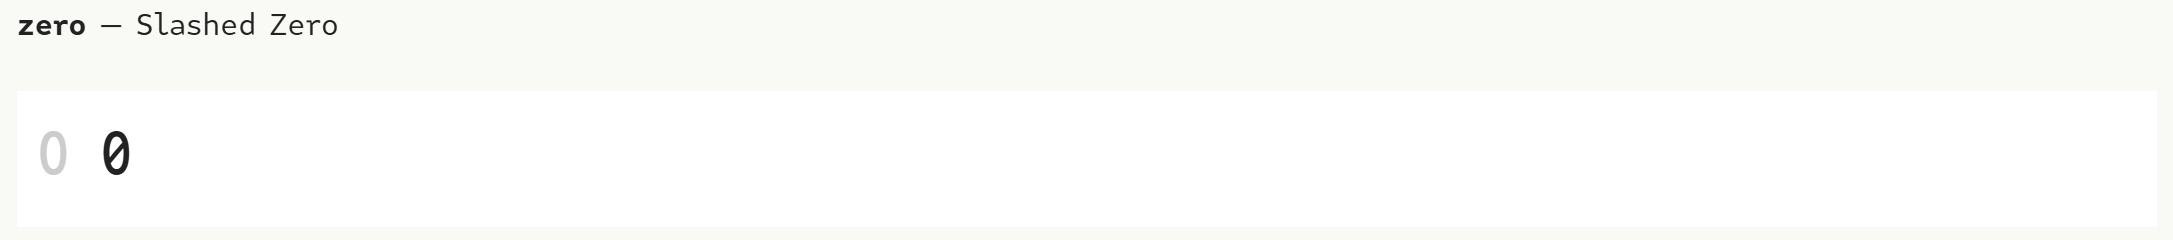
\includegraphics[width=0.625\linewidth]{pennstander_zero}

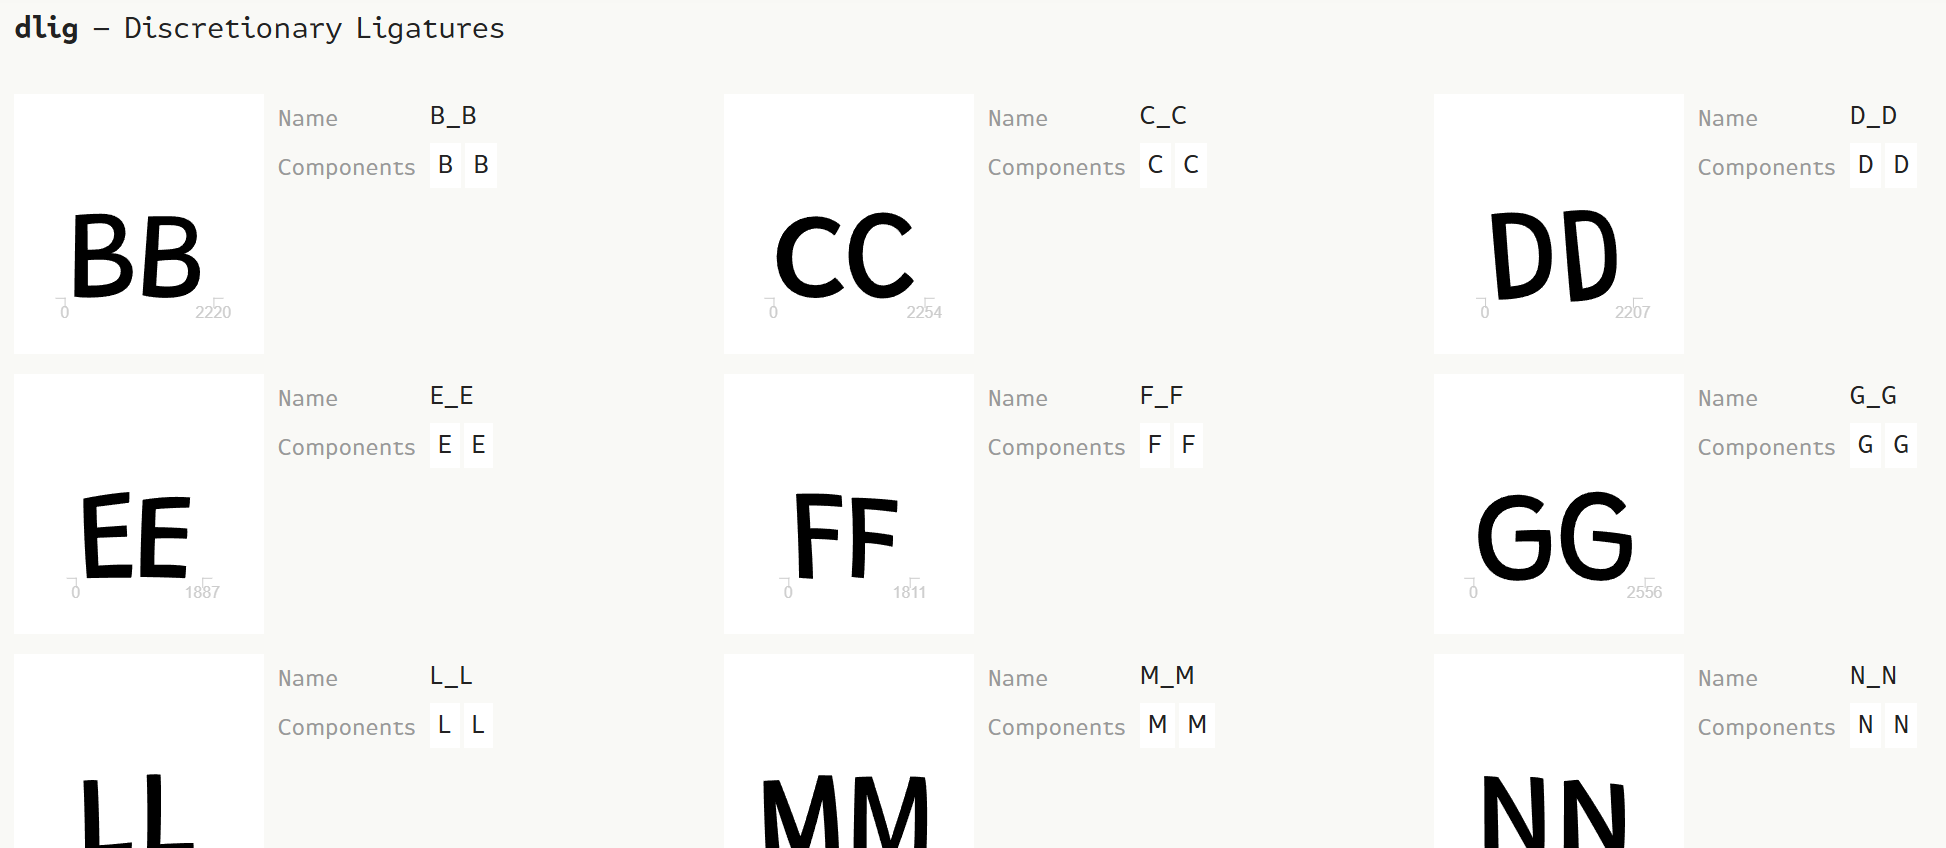
\includegraphics[width=0.625\linewidth]{pennstander_dlig}

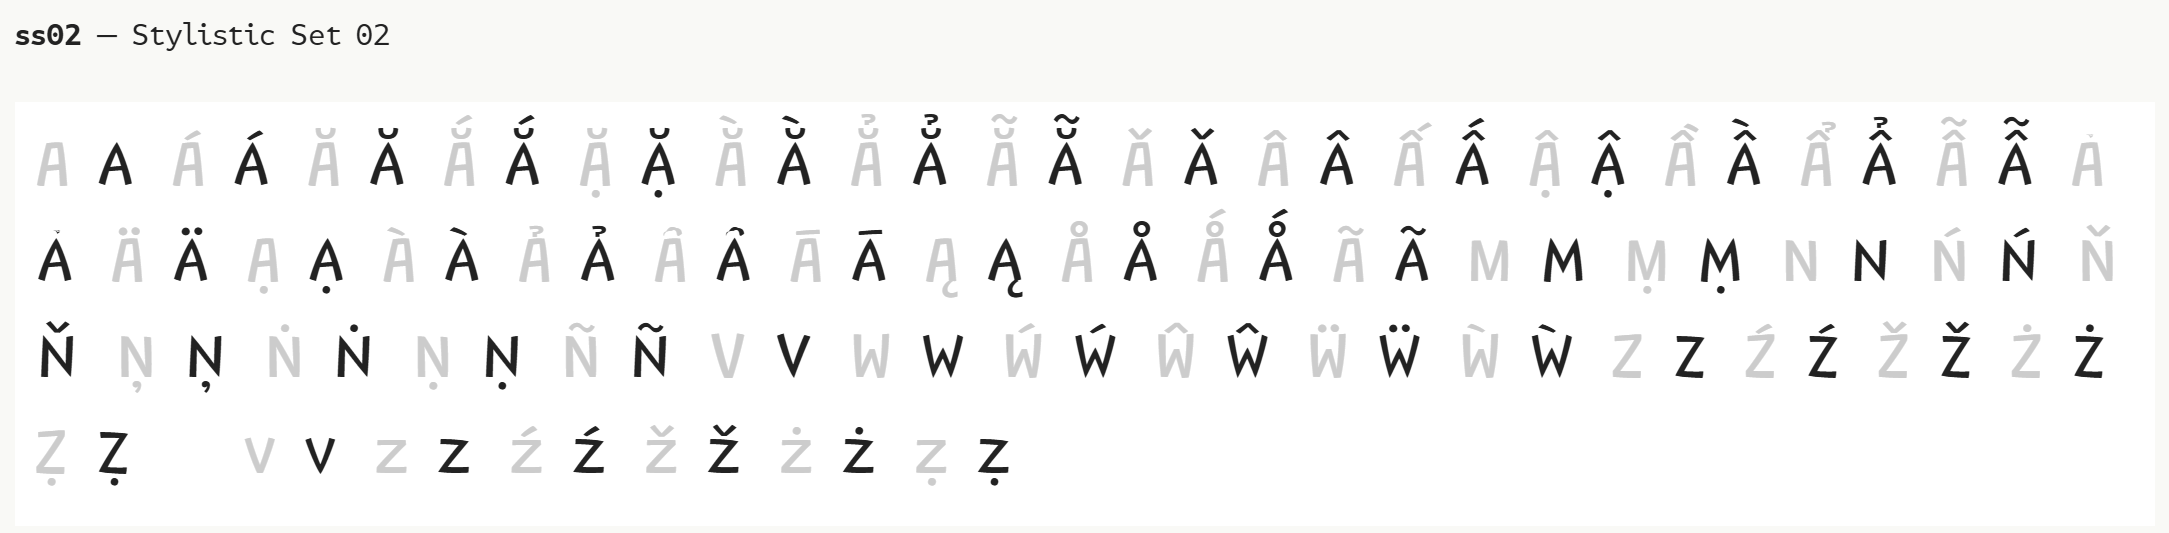
\includegraphics[width=0.625\linewidth]{pennstander_ss02}

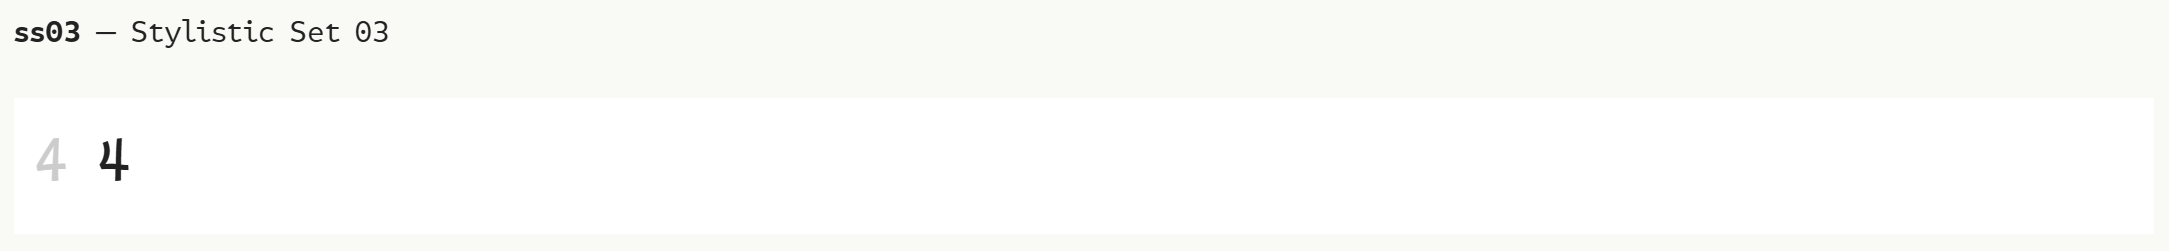
\includegraphics[width=0.625\linewidth]{pennstander_ss03}

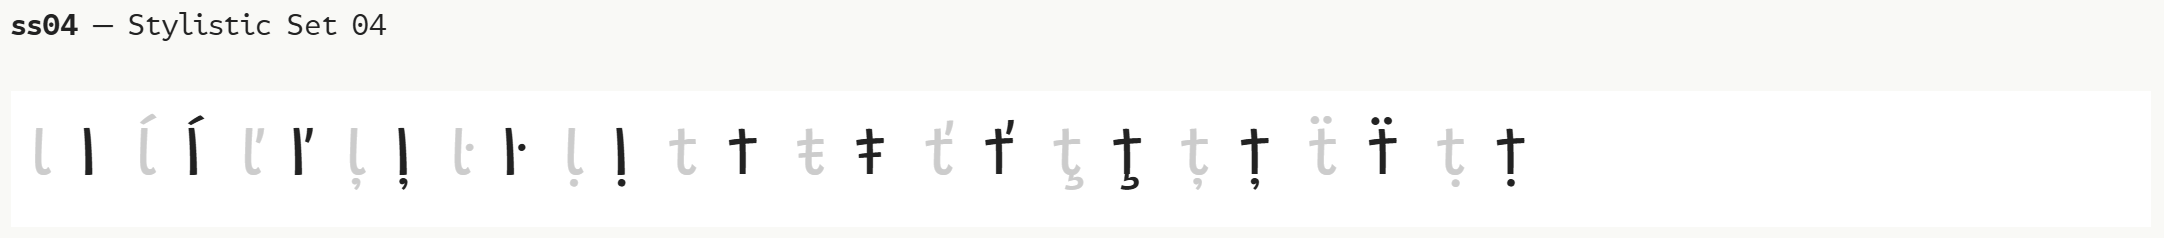
\includegraphics[width=0.625\linewidth]{pennstander_ss04}


\includegraphics[width=0.625\linewidth]{pennstander_ss06}

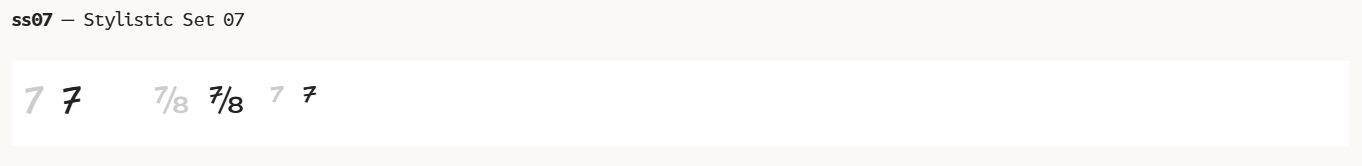
\includegraphics[width=0.625\linewidth]{pennstander_ss07}

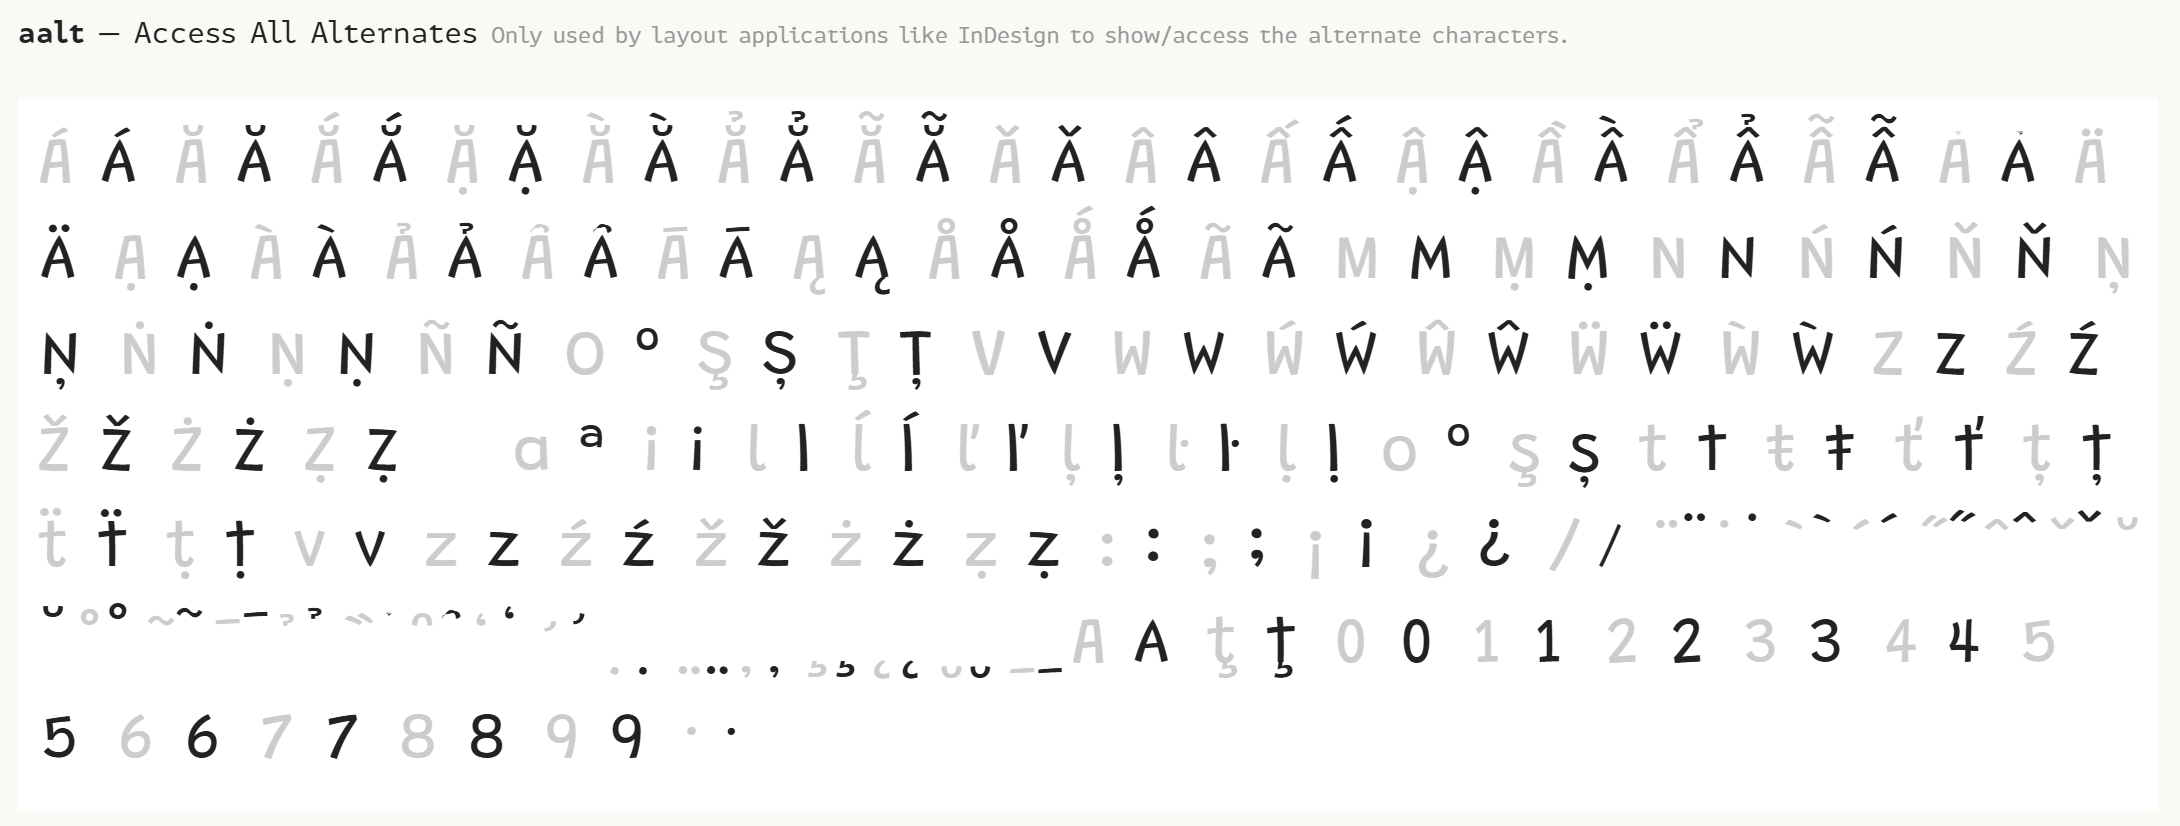
\includegraphics[width=0.625\linewidth]{pennstander_aalt}

\subsection{For math font}

Extra openfeatures for math font available are:

\begin{itemize}
	\item \opt{aalt}: Access All Alternatives
	\item \opt{dtls}: Dotless Forms
	\item \opt{zero}: Slashed Zero
	\item \opt{frac}: Fractions
	\item \opt{ss01}: Alternate a,g,I,Iota
	\item \opt{ss02}: Alternate A,M,N,Q,V,W,Z,v,z,Alpha,Mu,Rho,Zeta
	\item \opt{ss03}: Alternate 4
	\item \opt{ss04}: Alternate l,t
	\item \opt{ss05}: Simplified Fraktur A,K,L,X,Y,Z,x,y
	\item \opt{ss06}: Alternate ampersand
	\item \opt{ss07}: Alternate 7
\end{itemize}

\subsection{Unicode Private Use Area}

Glyphs assigned to Unicode Private Use Area:

\begin{itemize}
	\item Double-struck uppercase Greek letters: \opt{U+E1002–U+E1008}
	\item Fraction Rule: \opt{U+E000}
	\item Radical Rule: \opt{U+E001}
\end{itemize}

\pagebreak

\section{List of glyphs}

\subsection{Text version}

\displayfonttable{Pennstander-Regular}

\pagebreak

\subsection{Math version}

\displayfonttable[color=purple]{PennstanderMath-Regular}

\pagebreak

\section{Alphabets}

\subsection{Text version}

\textcolor{violet}{-- Normal/\textbf{Bold}/\textit{Italic}/\textit{\textbf{BoldItalic}}/\textsl{Slanted}/\textsl{\textbf{BoldSlanted}}:}

\abc\ABC\samplenumbers

\textbf{\abc\ABC\samplenumbers}

\textit{\abc\ABC\samplenumbers}

\textit{\textbf{\abc\ABC\samplenumbers}}

\textsl{\abc\ABC\samplenumbers}

\textsl{\textbf{\abc\ABC\samplenumbers}}

\smallskip

\textit{Slanted version uses italic version.}

\subsection{Math version}

\textcolor{violet}{-- Normal/\textbf{Bold}/\textit{Italic}/\textit{\textbf{BoldItalic}}:}

$\abc\ABC\samplenumbers$

$\mathbf{\abc\ABC\samplenumbers}$

$\mathit{\abc\ABC\samplenumbers}$

$\mathit{\mathbf{\abc\ABC\samplenumbers}}$

\smallskip

\textcolor{violet}{-- mathcal/mathfrak/mathbb:}

$\mathcal{\abc\ABC}$

$\mathfrak{\abc\ABC}$

$\mathbb{\ABC\samplenumbers}$

\end{document}